% M3 milestone: FR-9 required elements (diagram, image, Python graph, table, decorated formula).
% Paths are relative to latex/ (see ../figures/...).

\chapter{Required elements showcase (M3)}
\label{ch:m3_fr9}

This chapter exists so every FR-9 asset has a concrete \LaTeX{} anchor, caption, and
\texttt{\textbackslash label} for downstream cross-references (M4--M6).
Figure~\ref{fig:pipeline} is a native TikZ diagram.
Figure~\ref{fig:cover-art} is a raster image generated by \texttt{scripts/make\_image.py}.
Figure~\ref{fig:latency} is a vector graph from \texttt{scripts/make\_graph.py}.
Table~\ref{tab:requirements} summarizes contract checks.
Equation~\eqref{eq:normalized} mixes a matrix with a decorated piecewise update.

% --- Diagram (TikZ / vector, FR-9) ---
\begin{figure}[htbp]
\centering
\begin{tikzpicture}[
  font=\footnotesize,
  >=Stealth,
  node distance=11mm and 14mm,
  box/.style={draw, rounded corners=2pt, align=center, inner sep=4pt, minimum width=22mm},
]
  \node[box] (r) {Research\\\footnotesize sources + \texttt{.bib}};
  \node[box, right=of r] (o) {Outline\\\footnotesize page budget};
  \node[box, right=of o] (w) {Writer\\\footnotesize Markdown};
  \node[box, below=of o] (f) {Figures\\\footnotesize scripts $\rightarrow$ \texttt{figures/}};
  \draw[->, thick] (r) -- (o);
  \draw[->, thick] (o) -- (w);
  \draw[->, thick] (o) -- (f);
\end{tikzpicture}
\caption{Linear CrewAI document pipeline with a dedicated figure stage (TikZ).}
\label{fig:pipeline}
\end{figure}

% --- Image (raster, FR-9) ---
\begin{figure}[htbp]
\centering
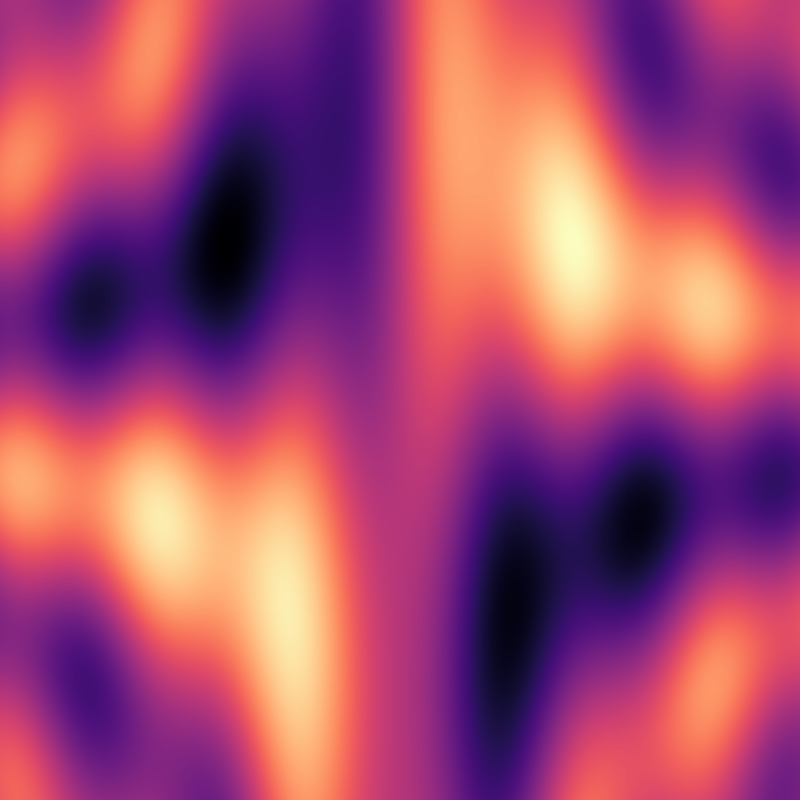
\includegraphics[width=0.36\linewidth]{../figures/image.png}
\caption{Thematic raster asset (Matplotlib \texttt{imshow}, deterministic field).}
\label{fig:cover-art}
\end{figure}

% --- Python-generated graph (vector PDF, FR-9) ---
\begin{figure}[htbp]
\centering
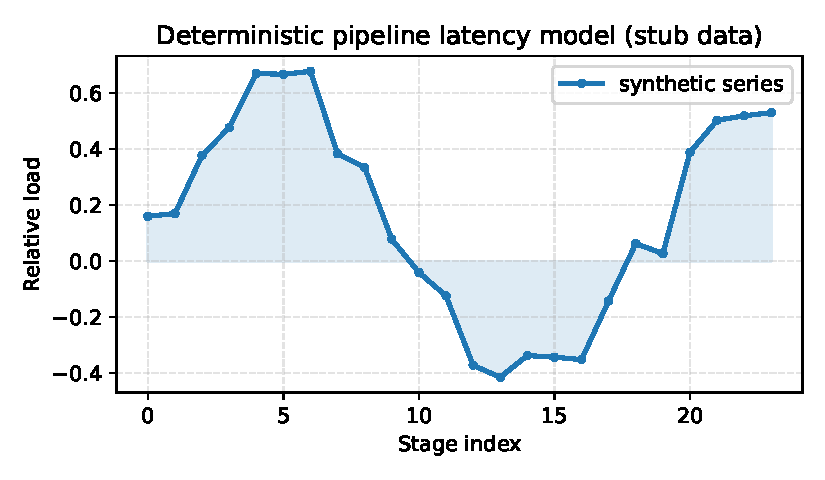
\includegraphics[width=0.62\linewidth]{../figures/graph.pdf}
\caption{Python/Matplotlib vector export (\texttt{figures/graph.pdf}).}
\label{fig:latency}
\end{figure}

% --- Table (FR-9) ---
\begin{table}[htbp]
\centering
\begin{tabular}{@{}lcc@{}}
\toprule
\textbf{Check} & \textbf{Target} & \textbf{Owner phase} \\
\midrule
Diagram present & TikZ or vector PDF & M3 \\
Python graph on disk & \texttt{figures/graph.pdf} & M3 \\
Raster image & \texttt{figures/image.png} & M3 \\
Decorated math & \texttt{equation} + matrix/cases & M3 \\
\bottomrule
\end{tabular}
\caption{FR-9 coverage matrix for graders (booktabs).}
\label{tab:requirements}
\end{table}

% --- Decorated equation (FR-9, FR-10) ---
\begin{equation}
\label{eq:normalized}
\mathbf{z}^{(t+1)} =
\begin{bmatrix}
\cos\theta & -\sin\theta \\
\sin\theta & \cos\theta
\end{bmatrix}
\mathbf{z}^{(t)}
+
\begin{cases}
\eta \,\nabla \mathcal{L}(\mathbf{z}^{(t)}), &
\lVert \nabla \mathcal{L}(\mathbf{z}^{(t)}) \rVert \le \tau, \\[6pt]
\eta \,\dfrac{\nabla \mathcal{L}(\mathbf{z}^{(t)})}
{\lVert \nabla \mathcal{L}(\mathbf{z}^{(t)}) \rVert}, &
\text{otherwise.}
\end{cases}
\end{equation}
